
\chapter{Experimentos e resultados}
% Label para referenciar
\label{experimentos-resultados}

% Diminuir espaçamento entre título e texto
\vspace{-1.9cm}

% Texto do capítulo

 Neste capítulo vamos abordar o ambiente de testes para os nossos protótipos e apresentar 
 o plano de testes utilizado e os resultados obtidos e análise dos dados.

\section{Ambiente de testes}
\label{ambientedetestes}

  Para efetuar os testes, os protótipos tiveram de ser colocados em uma ambiente de testes. 
  Para os dois protótipos, hospedamos a aplicação em uma VPS\footnote{http://digitalocean.com} da empresa Digital Ocean.
  
  O ambiente é composto pelos seguintes componentes de hardware conforme descrito nas tabelas\footnote{https://www.digitalocean.com/pricing/}
  de precificação do produto.
  
  \begin{table}[H]
    \centering
    \footnotesize
    % Alterar espaçamentos antes e depois do caption
    \setlength{\abovecaptionskip}{0pt}
    \setlength{\belowcaptionskip}{0pt}
    % Caption
    \caption[Componentes da VPS]{Componentes da VPS}
    \label{tab:components-digital-ocean-vps}
    % Conteúdo da tabela
    \begin{tabular}{c|c}
      \hline \hline
      Componente  &	Descrição \\
      \hline \hline
      Memória Ram & 512 MegaBytes \\
      Processador & 1 núcleo. \\
      Espaço em disco & 20 GigaBytes \ac{SSD}. \\
      Transferência em rede & 1 TeraByte. \\
      \hline \hline
    \end{tabular}
    % Fonte
    \captionfont{\small{\textbf{\\Fonte: Digital Ocean Pricing <https://www.digitalocean.com/pricing/> acesso 05. NOV. 2014}}}
  \end{table}

  Para os dois protótipos busca-se manter o máximo de igualdade entre os serviços executados, porém, por ser 
  tecnologias diferentes o modo de \textit{deploy} também são diferentes adicionando ou não novos serviços. 
  As informações dos serviços executados está listada de acordo com o software de monitoramento\footnote{http://newrelic.com}
  da empresa New Relic.
  
  A tabela \ref{tab:services-in-api-django} apresenta os serviços em execução do protótipo feito em Django sem clientes conectados.
  Este ambiente é composto por um servidor Nginx a execução do \textit{gunicorn},
  que nada mais é a execução do framework Django, o banco de dados Postgres 9.1 e o processo supervisord responsável por
  verificar se a aplicação esta ativa e caso ocorra alguma falha é capaz de reiniciar a aplicação.
  
  \begin{table}[H]
    \centering
    \footnotesize
    % Alterar espaçamentos antes e depois do caption
    \setlength{\abovecaptionskip}{0pt}
    \setlength{\belowcaptionskip}{0pt}
    % Caption
    \caption[Serviços executados na API Django]{Serviços executados na API Django}
    \label{tab:services-in-api-django}
    % Conteúdo da tabela
    \begin{tabular}{c|c|c}
      \hline \hline
      Processo  & 	CPU \% &	Memória \\
      \hline \hline
      gunicorn &	0.0\% &		104 MB \\
      postgres &	0.0\% &		19.3 MB \\
      supervisord &	0.0\% &		11.5 MB \\
      nginx &		0.0\% &		7.26 MB \\
      getty &		0.0\% &		5.69 MB \\
      udevd &		0.0\% &		4.05 MB \\
      nrsysmond &	0.1\% &		3.93 MB \\
      console-kit-dae &	0.0\% &		3.84 MB \\
      polkitd &	 	0.0\% &		2.98 MB \\
      ntpd &		0.0\% &		2.34 MB \\
      rsyslogd &	0.0\% &		1.47 MB \\
      nginx &		0.0\% &		1.38 MB \\
      sshd &		0.0\% &		1.22 MB \\
      dbus-daemon &	0.0\% &		1.13 MB \\
      cron &		0.0\% &		1.03 MB \\
      exim4 &		0.0\% &		992 KB \\
      init &		0.0\% &		820 KB \\
      acpid &		0.0\% &		656 KB \\
      atd &		0.0\% &		156 KB \\
      su &		0.0\% &		0 \\
      bash &		0.0\% &		0 \\
      \hline \hline
    \end{tabular}
    % Fonte
    \captionfont{\small{\textbf{\\Fonte: Autor}}}
  \end{table}
  
  \vspace{-1.9cm}

  Para o segundo protótipo, com Node.Js, possuimos os seguintes serviços executados na tabela \ref{tab:services-in-api-node}, 
  também sem nenhum cliente conectado. Este ambiente é composto por um servidor Nginx, o serviço \textit{pm2} responsável por
  verificar se a aplicação esta ativa e caso ocorra alguma falha é capaz de reiniciar a aplicação, 
  o banco de dados Postgres 9.1.
  
   \begin{table}[H]
    \centering
    \footnotesize
    % Alterar espaçamentos antes e depois do caption
    \setlength{\abovecaptionskip}{0pt}
    \setlength{\belowcaptionskip}{0pt}
    % Caption
    \caption[Serviços executados na API Node]{Serviços executados na API Node}
    \label{tab:services-in-api-node}
    % Conteúdo da tabela
    \begin{tabular}{c|c|c}
      \hline \hline
      Processo  & 	CPU \% &	Memória \\
      \hline \hline
      node &		0.0\% &		22.8 MB \\
      postgres &	0.0\% &		17.8 MB \\
      pm2 &		0.0\% &		17.4 MB \\
      nginx &		0.0\% &		6.61 MB \\
      getty &		0.0\% &		5.68 MB \\
      udevd &		0.0\% &		3.72 MB \\
      nrsysmond &	0.1\% &		3.93 MB \\
      rsyslogd &	0.0\% &		1.52 MB \\
      nginx &		0.0\% &		1.38 MB \\
      sshd &		0.0\% &		1.22 MB \\
      cron &		0.0\% &		1.02 MB \\
      exim4 &		0.0\% &		984 KB \\
      init &		0.0\% &		824 KB \\
      acpid &		0.0\% &		652 KB \\
      dbus-daemon &	0.0\% &		508 KB \\
      atd &		0.0\% &		152 KB \\
      su &		0.0\% &		0 MB \\
      console-kit-dae &	0.0\% &		0 MB \\
      startpar & 	0.0\% &		0 MB \\
      sshd &		0.0\% &		0 MB \\
      polkitd &		0.0\% &		0 MB \\
      \hline \hline
    \end{tabular}
    % Fonte
    \captionfont{\small{\textbf{\\Fonte: Autor}}}
  \end{table}
   
\subsection{Apresentação da ferramenta}
  
  Para realizar a simulação de múltiplos usuários na \ac{API} e obter os dados dos testes foi 
  escolhido o software como serviço da empresa SendGrid chamado loader.io. O loader.io é descrito em seu site
  como um simples serviço de teste de carga baseado em núvem. Em sua descrição tem-se a seguinte
  definição: Loader.io é um serviço de teste de carga, livre, que permite realizar um teste de estresse em 
  seus aplicativos web ou \textit{API\'s} com milhares de conexões simultâneas.
  
  Sua utilização é simples, basta criar uma conta com um e-mail válido. Após o e-mail ser validado pode-se 
  criar um teste dentre os 03 tipos já apresentados. Em resumo, temos os seguintes campos a serem preenchidos:
  
  \textbf{Nome do teste}: Nome dado ao teste para ser encontrado com maior facilidade;
  Tipo de teste: São apenas 03 tipos suportados pelo serviço. Clientes por teste, Clientes por segundo e Mantendo 
  a carga no servidor.
  
  \textbf{Autenticação}: Caso sua aplicação necessite de autenticação escolha a opção Autenticação Básica (tradução nossa),
  e setar os valores dos campos usuário e senha (tradução nossa). O serviço loader.io pede atenção 
  pois os campos, usuário e senha, não serão criptografados. Então é recomendado criar um usuário de teste na aplicação.
  
  \textbf{Conexões e Duração}: São as principais definições para o teste sendo que o campo duração
  é fixo em 60 segundos. As conexões serão explicadas na próxima sub-seção em conjunto com os tipos de teste.
  
  \textbf{Tempo limite e Erro}: Este campo especifica quanto tempo o teste irá esperar por uma resposta do aplicativo, antes
  de contar a requisição como erro. Por padrão é configurado para 10000 milessegundos ou 10 segundos.
  
  \textbf{Notas e etiquetas}: São campos para o desenvolvedor descrever  melhor os testes.
  
  \textbf{Urls e opções}: Configura a \ac{URL} que se deseja testar. Ha outras opções disponíveis como setar cabeçalhos \ac{HTTP},
  opções de resposta, váriaveis e outros que não serão utilizados neste trabalho.
  
  Para melhor entendimento do leitor e detalhamento é importante verificar 
  a documentação \footnote{http://support.loader.io/article/15-creating-a-test}.
  
\subsubsection{Tipos de teste}
  
  Os três tipos de testes suportados pelo serviço são:
  
  \textbf{Clientes no testes}
  
  Este teste permite que especifique um número total de clientes que se conectam ao serviço. Quando criar o teste,
  especifique somente um número de clientes então vários clientes irão se conectar ao longo da duração do teste. 
  Por exemplo, se for criado um teste com 20.000 clientes dentro de 20 segundos, o serviço irá executar a carga de 
  1.000 clientes por segundo. (tradução nossa)
  
  Em referência ao formulário de criação de teste o campo clientes representa o número de conexões que serão
  feitas para o servidor ao longo da duração do teste.
  
  \textbf{Clientes por segundo}
  
  Este teste permite que especifique um número de clientes que se conectam a cada segundo. Por exemplo se for criado
  um teste com 1.000 clientes dentro de 20 segundos, o serviço irá conectar 20.000 clientes neste teste.
  
  Em referência ao formulário de criação de teste o campo clientes representa o número de conexões que serão
  feitas para o servidor por segundo.
  
  \textbf{Mantendo carga do clientes}
  
  Segundo a definição da documentação, este teste é utilizado para sobrecarregar o site ou \ac{API}.
  
  O serviço loader.io garante que um número constante de clientes estará consumindo e realizando requisições em 
  sua \ac{API} a todo o momento.
  
  O teste inicia-se com um certo número de conexões ("de")  e pode aumentar as conexões ao longo do teste, 
  atingindo o número no campo "para", até ao final do teste. 
  
  Este teste permite que especifique um número mínimo e máximo de clientes. Especificando zero clientes
  até 10.000, por exemplo, o teste vai começar com zero até 10.000 clientes simultâneos no final do teste.
  
\subsubsection{Verificando o aplicativo}

  Após ter um entendimento base sobre os testes e como cadastra-los é necessário verficar a autenticidade do 
  aplicativo ou domínio para com o serviço Loader.io. Este processo só é feito uma vez. 
  
  O token fornecido pelo Loader.io pode ser verificado de duas maneiras.
  
  \textbf{Verificação por HTTP}.
  
  Pode-se realizar upload do arquivo loader-\textit{token} para o aplicativo e fazer com que a aplicação
  responda este arquivo texto através de uma rota com o mesmo nome do arquivo. 
  
  Para este trabalho, não foi feito upload do arquivo. Em vez disso, criamos a rota com o nome do token e
  na resposta da requisição \ac{HTTP} alteramos o cabeçalho do protocolo para \textit{text/plain} e imprimimos
  o valor do token.
  
  \textbf{Verificação por DNS.}
  
  A verificação ocorre quando o valor do token é inserido nas configurações de hospedagem através de um
  registro txt, com o valor \textit{loaderio=token}.
  
  Lembrando ao leitor que a propagação do \ac{DNS} pode levar algum tempo.
  
\subsubsection{Variáveis no Loader.io}

  As variáveis permitem usar dados de um cabeçalho de resposta \ac{HTTP} anterior e passa-los para o próximo
  teste.
  
  Como no exemplo da documentação do loader.io, em uma requisição do tipo \textit{GET} foi configurada uma váriavel
  com a chave \ac{CSRF} e o respectivo valor de cabeçalho \textit{X-Csrf-Token}. Em seguida em uma requisição 
  do tipo \textit{POST} foi utilizada essa chave-valor através da variável com o nome \textit{authenticity token} e valor
  \textit{\{\{csrf\}\}}.
  
  Essa opção de uso de váriaveis não foi utilizada em nossos testes mas é importante relatar ao leitor que
  é existe tais funcionalidades na ferramenta.

  
\subsubsection{Resultados dos testes}

  Para cada execução de teste gera-se um resultado. Veja abaixo um sumário de cada campo para melhor interpretação.
  
  \begin{compactitem}
    \item[a)] Date e Time: Data e hora de quando o teste foi executado.
    \item[b)] Max users: Número máximo de conexões que foram feitas.
    \item[a)] Duration:  Duração do teste.
    \item[a)] Success response: O número total de resposta com staus code (1xx,2xx,3xx).
    \item[a)] Avg responses time: Tempo médio que o aplicativo esperou por uma resposta do aplicativo.
    \item[a)] Sent from app: Quantidade total em MegaBytes enviados para o aplicativo.
    \item[a)] RCVD from loader: Quantidade total em MegaBytes foi recebida pelo aplicativo.
    \item[a)] Timeout errors: Número de pedidos que não receberam uma resposta dentro do tempo limite configurado.
    \item[a)] Network errors: Erros da camada de transporte e de rede como \ac{DNS}, \textit{timeouts} de conexão TCP, dentre outros.
    \item[a)] Errors(400/500): Respostas das requisições com um código de erro (4xx e 5xx).
    \item[a)] Avg error rate: Porcentagem de erros do total de tentativas dos pedidos.
  \end{compactitem}

  \textbf{Gráficos}
  
  São três tipos de gráficos disponibilizados pelo Loader.io que oferecem informações mais detalhadas 
  sobre o que ocorreu na execução do teste como tempos de resposta, taxas de erro e largura de banda.
  
  \textbf{O gráfico temporal}.
  
  Gráfico que exibe os tempos de resposta apresentando duas linhas.
  
  Em verde, tem-se o número de conexões realizadas no aplicativo. E em azul é o tempo médio de resposta das
  requisições.
  
  \textbf{O gráfico de detalhes.}
  
  O gráfico que exibe taxas de sucesso e também de erros. Seu objetivo é exibir quando o aplicativo
  começa a disparar os erros.
  
  \textbf{O gráfico largura de banda.}
  
  Este gráfico mostra o quanto os dados foram enviados a partir do seu aplicativo.


\section{Testes}

  Descreve-se nesta seção os planos de testes utilizado em cada tipo de teste e a interpretação dos seus resultados
  através de comparação.
  
  Foi utilizada a seguinte nomenclatura para os testes com o aplicativo Django. Primeiramente teremos a letra (A) para identificar
  que o plano de teste será executado para o aplicativo Django. Em seguida temos a sequência númerica de 01 a 03, 
  identificando o testes realizados. 
  
  No aplicativo Node.Js utilizamos o mesmo padrão descrito no paragráfo anterior alterando apenas a letra inicial para (B) identificando
  que os testes foram realizados para o aplicativo em Node.Js.
  
  Por padrão da ferramenta e para a consciencia do leito o erro de tempo limite ocorre após 10 segundos e a execução do teste é abortada
  ao receber uma taxa de erro acima de 50\% (porcento). Essa taxa de erro é contabilizada somando os erros de tempo de limite, erros de 
  rede, erros com status de respota do protocolo \ac{HTTP} 400 ou 500.
  
  A visualização dos resultados foi sumarizada em uma nova tabela e foi gerado os gráficos a partir dela para apresentação dos
  dados ao leitor.
  
\subsection{Clientes por teste}  

  
  Apresenta-se nesta seção o plano de teste A-1 e B-1 que corresponde ao teste clientes por teste o qual tem-se um sumário
  de conexões com sucesso distruibuídos em 1 minuto de execução.
  
  Ao inciar este teste, foi estipulado que o número de conexões com sucesso deve começar por 1000 sucessos aumentando
  em mais 1000 sucessos até que ferramenta aborte o teste ao atingir a taxa de erro estipulada. Para cada teste
  foi executado 7 vezes e destes resultados retiramos a média para o tempo de resposta, número de sucessos, erro de tempo de limite e
  e a média para erros de rede.
  
  Veja o exemplo do teste A-3.1 o qual obtivemos os dados gerados pela ferramenta
  
  \begin{table}[H]
    \centering
    \footnotesize
    % Alterar espaçamentos antes e depois do caption
    \setlength{\abovecaptionskip}{0pt}
    \setlength{\belowcaptionskip}{0pt}
    % Caption
    \caption[Teste A-1.1 com a API Django 1000 clientes]{Teste A 1.1 com a API Django 1000 clientes}
    \label{tab:teste-a-1-1}
    % Conteúdo da tabela
    \begin{tabular}{c|c|c|c|c}
      \hline \hline
      Número de execução &	Tempo médio de resposta &	Número de sucessos &	Timeout Error &		 Network Errors&	Avg Error Rate \% \\
      \hline \hline
      Primeira execução &		121 &				1000 &			0 &			0 &			0 \\
      Segunda execução &		111 &				1000 &			0 &			0 &			0 \\
      Terceira execução &		119 &				1000 &			0 &			0 &			0 \\
      Quarta execução  &		88 &				1000 &			0 &			0 &			0 \\
      Quinta execução  &		90 &				999 &			1 &			0 &			0 \\
      Sexta execução   &		116 &				1000 &			0 &			0 &			0 \\
      Sétima execução  &		104 &				1000 &			0 &			0 &			0 \\
      Media & 				107 &				999.85 & 		0 &			0 &			0 \\
      \hline \hline
    \end{tabular}
    % Fonte
    \captionfont{\small{\textbf{\\Fonte: Autor}}}
  \end{table}  
  
  A tabela \ref{tab:teste-a-1-1} mostra que na primeira execução do teste A-1.1 com 1000 sucessos de conexões de clientes
  durante 1 minuto de duração obteve-se 121 milesegundos no tempo médio de resposta,
  1000 números de sucessos, 0 erros de tempo de limite, 0 erros de rede. Somente na quinta execução o número de sucessos
  caiu para 999 e houve um erro de limite de tempo.
  
  Para este plano de teste A-1, foram realizados as séries A-1.1 com 1000 clientes, A-1.2 com 2000 clientes, A-1.3 com 3000 clientes,
  A-1.4 com 4000 clientes. Após estes valores o Django apresentou altos indices de erros ultrapassando o valor de taxa de erro
  aceitável de 50 \%. Com os dados obtidos de cada teste pode-se fazer o sumário
  destes que serão apresentados a seguir na tabela \ref{tab:sumario-resultado-plano-teste-a-1}.
  
   
  \begin{table}[H]
    \centering
    \footnotesize
    % Alterar espaçamentos antes e depois do caption
    \setlength{\abovecaptionskip}{0pt}
    \setlength{\belowcaptionskip}{0pt}
    % Caption
    \caption[Sumário dos resultados do plano A-1]{Sumário dos resultados do plano A-1	}
    \label{tab:sumario-resultado-plano-teste-a-1}
    % Conteúdo da tabela
    \begin{tabular}{c|c|c|c|c}
      \hline \hline
      Intervalos  & 	Média de tempo de resposta (ms) \% &	Número de sucessos & 	Erro de tempo de limite &	Erro de rede \\ 
      \hline \hline
      1000 &		107 &					999.8571428571 & 		0.1428571429 &			0 \\
      2000 &		118.4285714286 &			1999.7142857143 & 		0.2857142857  &			0 \\
      3000 &		3737.7142857143 &			2405.8571428572 & 		301.1428571429 &		0 \\
      4000 &		6771 &					1792.5714285714 & 		1574.4285714286 &		0 \\
      \hline \hline
    \end{tabular}
    % Fonte
    \captionfont{\small{\textbf{\\Fonte: Autor}}}
  \end{table}
  
  A tabela \ref{tab:sumario-resultado-plano-teste-a-1} exibe as médias dos campos (média de tempo de resposta, 
  média do número de sucessos, média de erros de tempo de limite, média de erros de rede) de cada teste executado 
  para o plano de teste A-1 do protótipo Django.
  
  Com os dados acima foi possível gerar o gráfico \ref{grafico:teste-clientes-por-teste-django} do 
  prtótipo Django.
  
  \begin{grafico}[H]
    % Alterar espaçamentos antes e depois do caption
    \setlength{\abovecaptionskip}{5pt}
    \setlength{\belowcaptionskip}{0pt}
    \label{grafico:teste-clientes-por-teste-django}
    % Caption
    \caption[Clientes por teste no Django]
	    {Clientes por teste no Django}
    \centering
    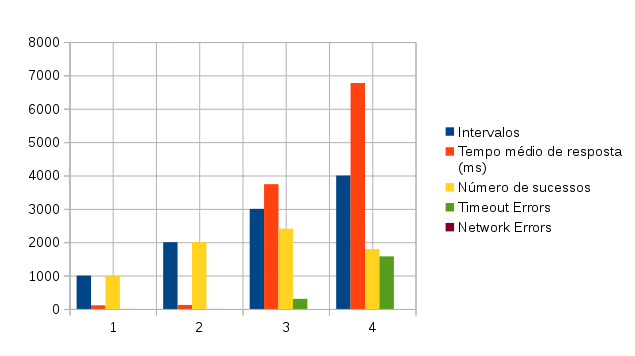
\includegraphics[width=.80\textwidth]{imagem/graficos/grafico_django_plano_de_teste_1.png}
    % Caption centralizada
    \captionsetup[grafico]{justification=centering}
    % Fonte
    \captionfont{\small{\textbf{\\Fonte: Autor}}}
  \end{grafico}
  
  Na interpretação do gráfico \ref{grafico:teste-mantendo-carga-usuario-django}  observa-se que com baixos números de sucessos foram 
  até 4000 mas possuindo uma perda significativa de desempenho. Entre 1000 a 2000 clientes por teste a aplicação se comportou muito bem
  com o tempo de resposta entre 107 a 118 e número de sucessos entre 999 e 1999 respectivamente; pode-se observar também que houve poucos
  erros de tempo limite excedido. A partir do valores de 3000 clientes por segundo os valores de tempo de resposta subiu drasticamente
  com importância no teste com 4000 clientes, pois, o tempo de resposta foi de 6771 milessegundos algo em torno de 6,76 segundos com um 
  baixo número de sucessos, menor até do que o plano de teste A.1.2 que foi em média de 1792 para 1999 respectivamente. Além do alto indice
  de tempo limite excedido no plano de teste A.1.4.
  
  Seguindo o mesmo modelo e conceitos de teste adotado para o protótipo Django, foi aplicado no plano de teste 
  B-1 correlacionando ao protótipo Node.Js. 
  
  A partir do exemplo do teste B-1.1 o qual obtivemos os dados gerados pela ferramenta, já é possível comparar a eficiência das 
  tecnologias empregadas em cada protótipo.
  
  \begin{table}[H]
    \centering
    \footnotesize
    % Alterar espaçamentos antes e depois do caption
    \setlength{\abovecaptionskip}{0pt}
    \setlength{\belowcaptionskip}{0pt}
    % Caption
    \caption[Teste B-1.1 com a API 1000 clientes]{Teste B 1.1 com a API Node.Js 1000 clientes}
    \label{tab:teste-b-1-1}
    % Conteúdo da tabela
    \begin{tabular}{c|c|c|c|c}
      \hline \hline
      Intervalos  & 	Média de tempo de resposta (ms) \% &	Número de sucessos & 	Erro de tempo de limite &	Erro de rede \\ 
      \hline \hline
      1000 &		12.5714285714 &				1000 & 				0 &				0 \\
      2000 &		12.4285714286 &				2000 & 				0 &				0 \\
      3000 &		12.1428571429 &				3000 & 				0 &				0 \\
      4000 &		12 &					4000 & 				0 &				0 \\
      5000 &		12.4285714286 &				5000 & 				0 &				0 \\
      6000 &		12.4285714286 &				6000 & 				0 &				0 \\
      7000 &		12.1428571429 &				7000 & 				0 &				0 \\
      8000 &		12.2857142857 &				7998.28 & 			0 &				0 \\
      9000 &		12.8571428571 &				9000 & 				0 &				0 \\
      10000 &		13.7142857143 &				9996.28 &		 	0 &				0 \\
      \hline \hline
    \end{tabular}
    % Fonte
    \captionfont{\small{\textbf{\\Fonte: Autor}}}
  \end{table}
  
  A tabela \ref{tab:teste-a-1-1} mostra que na primeira execução do teste A-1.1 com 1000 sucessos de conexões de clientes
  durante 1 minuto de duração obteve-se 12 milesegundos no tempo médio de resposta,
  1000 números de sucessos, 0 erros de tempo de limite, 0 erros de rede.
  
  Outro dado importante a ser salientado é que no plano de teste B-1 conseguiu alcançar o limite máximo suportado pela ferramenta
  loader.io chegando aos 10000 clientes por testes. Aqui já podemos comprovar a eficiencia do Node.Js em responder mais conexões que
  o protótipo Django. Sendo assim a série de teste ficou: B-1.1 com 1000 clientes, B-1.2 2000 clientes, 
  B-1.3 com 3000 clientes, B-1.4 com 4000 clientes, B-1.5 com 5000 clientes, B-1.6 com 6000 clientes, B-1.7 com 7000 clientes,
  B-1.8 com 8000 clientes, B-1.9 com 9000 clientes e B-1.10 com 10000 clientes. Com estes dados obtidos de cada teste pode-se fazer 
  o sumário destes que serão apresentados a seguir na tabela \ref{tab:sumario-resultado-plano-teste-b-1}.
  
  \begin{table}[H]
    \centering
    \footnotesize
    % Alterar espaçamentos antes e depois do caption
    \setlength{\abovecaptionskip}{0pt}
    \setlength{\belowcaptionskip}{0pt}
    % Caption
    \caption[Sumário dos resultados do plano B-1]{Sumário dos resultados do plano B-1}
    \label{tab:sumario-resultado-plano-teste-b-1}
    % Conteúdo da tabela
    \begin{tabular}{c|c|c|c|c}
      \hline \hline
      Intervalos  & 	Média de tempo de resposta (ms) \% &	Número de sucessos & 	Erro de tempo de limite &	Erro de rede \\ 
      \hline \hline
      1000 &		12.5714285714 &	 				1000 & 	 		0 &				0 \\
      2000 &		12.4285714286 &					2000 & 	 		0 &				0 \\
      3000 &		12.1428571429 &					3000 & 	 		0 &				0 \\
      4000 &		12  &						4000 & 	 		0 &				0 \\
      5000 &		12.4285714286  &				5000 & 	 		0 &				0 \\
      6000 &		12.4285714286 &					6000 & 	 		0 &				0 \\
      7000 &		12.1428571429 &					7000 & 	 		0 &				0 \\
      8000 &		12.2857142857 &					7998 & 	 		0 &				0 \\
      9000 &		12.8571428571 &					9000 & 	 		0 &				0 \\
      10000 &		13.7142857143 &					9996 & 	 		0 &				0 \\
      \hline \hline
    \end{tabular}
    % Fonte
    \captionfont{\small{\textbf{\\Fonte: Autor}}}
  \end{table}
   
  Assim como a tabela \ref{tab:sumario-resultado-plano-teste-a-1}, esta tabela \ref{tab:sumario-resultado-plano-teste-b-1} exibe as médias 
  dos campos (média de tempo de resposta, média do número de sucessos, média de erros de tempo de limite, média de erros de rede) 
  de cada teste executado para o plano de teste B-1 do protótipo Node.Js.
  
  Comparando as duas tabelas \ref{tab:sumario-resultado-plano-teste-a-1} e \ref{tab:sumario-resultado-plano-teste-b-1}, pode-se ver que 
  o tempo de resposta com o protótipo Node.Js fica em torno de 12 a 13 milessegundos ao contrario dos dados da tabela \ref{}
  
  Com os dados acima foi possível gerar o gráfico \ref{grafico:teste-mantendo-carga-usuario-node} referente aos testes 
  realizados com o Node.Js

  \begin{grafico}[H]
    % Alterar espaçamentos antes e depois do caption
    \setlength{\abovecaptionskip}{5pt}
    \setlength{\belowcaptionskip}{0pt}
    \label{grafico:teste-mantendo-carga-usuario-node}
    % Caption
    \caption[Mantendo a carga de usuários no Node.Js]
	    {Mantendo a carga de usuários no Node.Js}
    \centering
    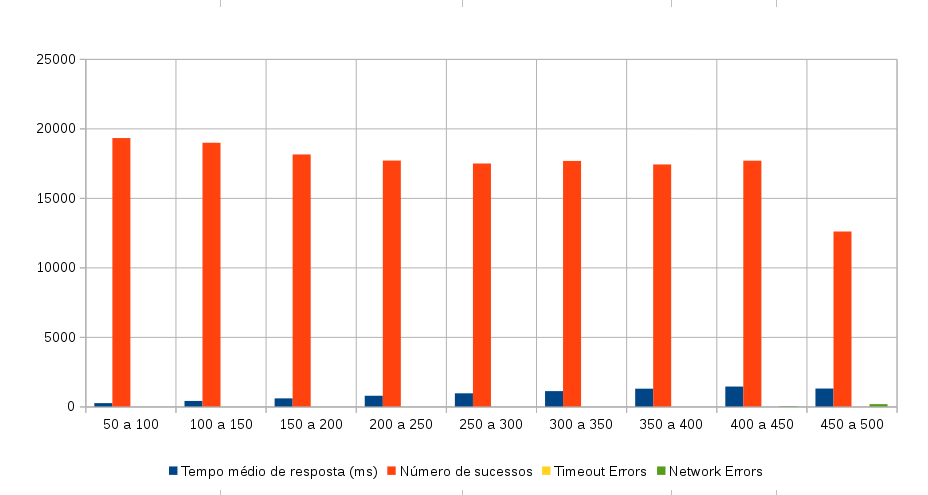
\includegraphics[width=.80\textwidth]{imagem/graficos/grafico_node_plano_de_teste_3.png}
    % Caption centralizada
    \captionsetup[grafico]{justification=centering}
    % Fonte
    \captionfont{\small{\textbf{\\Fonte: Autor}}}
  \end{grafico}
   
\subsection{Clientes por segundo}  


    
\subsection{Manter a carga no Servidor}  

    
  Apresenta-se nesta seção o plano de teste A-3 e B-3 que corresponde ao teste manter carga de usuários o qual tem-se um sumário
  com as médias de cada execução.
  
  Para melhor instruir o leitor, esse teste inicia com 50 a 100 usuários conectados no sistema até 1 minuto de duração. Para cada teste
  foi executado 7 vezes e destes resultados retiramos a média para o tempo de resposta, número de sucessos, erro de tempo de limite e
  e a média para erros de rede. No decorrer da série acrescentamos 50 usuários até a quantidade máxima suportada pela aplicação.
  
  Veja o exemplo do teste A-3.1 o qual obtivemos os dados gerados pela ferramenta.
  
  \begin{table}[H]
    \centering
    \footnotesize
    % Alterar espaçamentos antes e depois do caption
    \setlength{\abovecaptionskip}{0pt}
    \setlength{\belowcaptionskip}{0pt}
    % Caption
    \caption[Teste A-3.1 com a API Django 50 – 100 clientes]{Teste A 3.1 com a API Django 50 – 100 clientes}
    \label{tab:teste-a-3-1}
    % Conteúdo da tabela
    \begin{tabular}{c|c|c|c|c}
      \hline \hline
      Número de execução &	Tempo médio de resposta &	Número de sucessos &	Timeout Error &		 Network Errors&	Avg Error Rate \% \\
      \hline \hline
      Primeira execução &	1605 &				2754 &			0 &				0 &		0 \\
      Segunda execução &	1661 &				2659 &			0 &				0 &		0 \\
      Terceira execução &	1691 &				2610 &			0 &				0 &		0 \\
      Quarta execução  &	1678 &				2631 &			0 &				0 &		0 \\
      Quinta execução  &	1652 &				2674 &			0 &				0 &		0 \\
      Sexta execução   &	1634 &				2712 &			0 &				0 &		0 \\
      Sétima execução  &	1628 &				2707 &			0 &				0 &		0 \\
      Media & 			1649.8571428572 &		2678.1428571429 & 	0 &				0 &		0 \\
      \hline \hline
    \end{tabular}
    % Fonte
    \captionfont{\small{\textbf{\\Fonte: Autor}}}
  \end{table}
  
  A tabela \ref{tab:teste-a-3-1} mostra que na primeira execução do teste A-3.1 com o minimo de 50 clientes até o máximo de 100 clientes
  durante 1 minuto de duração obteve-se 1605 milesegundos no tempo médio de resposta,
  2754 números de sucessos, 0 erros de tempo de limite, 0 erros de rede.
  
  Para este plano de teste A-3, foram realizados as séries A-3.1 de 50 a 100 clientes, A-3.2 de 100 a 150 clientes, A-3.3 de 150 a 200 clientes,
  A-3.4 de 200 a 250 clientes, A-3.5 de 250 a 300, A-3.6 de 300 e 350 clientes. Com os dados obtidos de cada teste pode-se fazer o sumário
  destes que serão apresentados a seguir na tabela \ref{tab:sumario-resultado-plano-teste-a-3}.
  
  \begin{table}[H]
    \centering
    \footnotesize
    % Alterar espaçamentos antes e depois do caption
    \setlength{\abovecaptionskip}{0pt}
    \setlength{\belowcaptionskip}{0pt}
    % Caption
    \caption[Sumário dos resultados do plano A-3]{Sumário dos resultados do plano A-3}
    \label{tab:sumario-resultado-plano-teste-a-3}
    % Conteúdo da tabela
    \begin{tabular}{c|c|c|c|c}
      \hline \hline
      Intervalos  & 	Média de tempo de resposta (ms) \% &	Número de sucessos & 	Erro de tempo de limite &	Erro de rede \\ 
      \hline \hline
      50 a 100 &		1649.8571428572 &		2678.1428571429 & 	0 &				0 \\
      100 a 150&		2663.1428571429 &		2734.2857142857 & 	2.8571428571  &			0 \\
      150 a 200&		5539.8571428572 &		1487.4285714286 & 	258.8571428571 &		0 \\
      200 a 250&		5452.2857142857 &		1714.4285714286 & 	574.4285714286 &		0 \\
      250 a 300&		5964.1428571429 &		1717.5714285714 & 	810.5714285714 &		0 \\
      300 a 350&		6256.7142857143 &		1625.8571428572 & 	935.2857142857 &		0 \\
      \hline \hline
    \end{tabular}
    % Fonte
    \captionfont{\small{\textbf{\\Fonte: Autor}}}
  \end{table}
   
  A tabela \ref{tab:sumario-resultado-plano-teste-a-3} exibe as médias dos campos (média de tempo de resposta, 
  média do número de sucessos, média de erros de tempo de limite, média de erros de rede) de cada teste executado 
  para o plano de teste A-3 do protótipo Django.
  
  Com os dados acima foi possível gerar o gráfico \ref{grafico:teste-mantendo-carga-usuario-django} do 
  prtótipo Django.
  
  \begin{grafico}[H]
    % Alterar espaçamentos antes e depois do caption
    \setlength{\abovecaptionskip}{5pt}
    \setlength{\belowcaptionskip}{0pt}
    \label{grafico:teste-mantendo-carga-usuario-django}
    % Caption
    \caption[Mantendo a carga de usuários no Django]
	    {Mantendo a carga de usuários no Django}
    \centering
    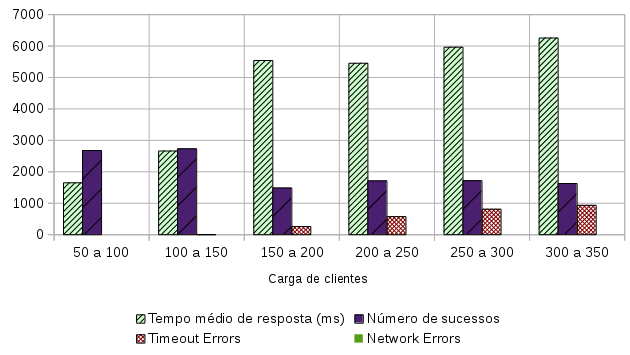
\includegraphics[width=.80\textwidth]{imagem/graficos/grafico_django_plano_de_teste_3.png}
    % Caption centralizada
    \captionsetup[grafico]{justification=centering}
    % Fonte
    \captionfont{\small{\textbf{\\Fonte: Autor}}}
  \end{grafico}
  
  Ao interpretar o gráfico \ref{grafico:teste-mantendo-carga-usuario-django}  observa-se que com baixos números de clientes 
  conectados no sistema tem-se um tempo de resposta menor para um alto número de sucessos. Ao elevar o número minimo e máximo de 
  clientes conectados observa-se que o tempo de resposta foi quase o mesmo do número de sucessos. Com novos acréscimos de usuários
  no protótipo elevando o número minimo e máximo de clientes conectados pode-se observar que o tempo médio de resposta foi elevado
  em grandes números e o número de sucessos de cada requisição abaixou em comparação ao primeiro teste. Também é possível verificar,
  que com o aumento de usuários houve a incidência de erros de tempo de limite nas conexões.
  
  Este teste prova que o protótipo Django possui pouca eficiência em lidar com usuários conectados ao sistema. Veja que os tempos de 
  resposta são altos e o número de sucessos são baixos para uma aplicação simples cujo objetivo é somente consumir as informações do banco de 
  dados através do método \textit{GET} da API.
  
  Seguindo o mesmo modelo e conceitos de teste adotado para o protótipo Django, foi aplicado no plano de teste 
  B-3 correlacionando ao protótipo Node.Js. 
  
  A partir do exemplo do teste B-3.1 o qual obtivemos os dados gerados pela ferramenta, já é possível comparar a eficiência das 
  tecnologias empregadas em cada protótipo.
  
  \begin{table}[H]
    \centering
    \footnotesize
    % Alterar espaçamentos antes e depois do caption
    \setlength{\abovecaptionskip}{0pt}
    \setlength{\belowcaptionskip}{0pt}
    % Caption
    \caption[Teste B-3.1 com a API Node.Js 50 – 100 clientes]{Teste B 3.1 com a API Node.Js 50 – 100 clientes}
    \label{tab:teste-b-3-1}
    % Conteúdo da tabela
    \begin{tabular}{c|c|c|c|c}
      \hline \hline
      Número de execução &	Tempo médio de resposta &	Número de sucessos &	Timeout Error &		 Network Errors&	Avg Error Rate \% \\
      \hline \hline
      Primeira execução &	229 &				19632 &			0 &				0 &		0 \\
      Segunda execução &	230 &				19514 &			0 &				0 &		0 \\
      Terceira execução &	233 &				19282 &			0 &				0 &		0 \\
      Quarta execução  &	230 &				19486 &			0 &				0 &		0 \\
      Quinta execução  &	235 &				19103 &			0 &				0 &		0 \\
      Sexta execução   &	231 &				19389 &			0 &				0 &		0 \\
      Sétima execução  &	240 &				18724 &			0 &				0 &		0 \\
      Media & 			232.5714285714 &		19304.2857142857 & 	0 &				0 &		0 \\
      \hline \hline
    \end{tabular}
    % Fonte
    \captionfont{\small{\textbf{\\Fonte: Autor}}}
  \end{table}
  
  A tabela \ref{tab:teste-b-3-1} mostra que na primeira execução do teste B-3.1 com o minimo de 50 clientes até o máximo de 100 clientes
  durante 1 minuto de duração. Para este teste obteve-se 232 milesegundos no tempo médio de resposta, valor muito inferior ao do plano de
  teste A-3.1 da tabela \ref{tab:teste-a-3-1} o qual foi de 1649.8571428572 milsesegundos, significando que a resposta para os usuários
  foi bem mais rápida do que o protótipo em Django. Vale ressaltar que o número de sucessos para cada conexão ficou em média de 
  19304.2857142857, número superior ao teste A-3.1 de apenas 2754 números de sucessos.
  
  Outro dado importante a ser salientado é que no plano de teste B-3 conseguiu alcançar o limite de 450 a 500 usuários conectados
  na aplicação durante 1 minuto de duração. Valor este superior ao do plano de teste A-3 em que o limite de usuário chegou a apenas
  de 300 a 350 usuários conectados. Sendo assim a série de teste ficou B-3.1 de 50 a 100 clientes, B-3.2 de 100 a 150 clientes, 
  B-3.3 de 150 a 200 clientes, B-3.4 de 200 a 250 clientes, B-3.5 de 250 a 300, B-3.6 de 300 e 350 clientes, B-3.7 de 350 a 400 clientes,
  B-3.8 de 400 a 450 clientes, B-3.9 de 450 a 500 clientes. A partir deste número de clientes houve uma taxa de erro superior ao
  configurado na ferramenta. Com estes dados obtidos de cada teste pode-se fazer o sumário
  destes que serão apresentados a seguir na tabela \ref{tab:sumario-resultado-plano-teste-b-3}.
  
  \begin{table}[H]
    \centering
    \footnotesize
    % Alterar espaçamentos antes e depois do caption
    \setlength{\abovecaptionskip}{0pt}
    \setlength{\belowcaptionskip}{0pt}
    % Caption
    \caption[Sumário dos resultados do plano B-3]{Sumário dos resultados do plano B-3}
    \label{tab:sumario-resultado-plano-teste-b-3}
    % Conteúdo da tabela
    \begin{tabular}{c|c|c|c|c}
      \hline \hline
      Intervalos  & 	Média de tempo de resposta (ms) \% &	Número de sucessos & 	Erro de tempo de limite &	Erro de rede \\ 
      \hline \hline
      50 a 100 &		232.5714285714  &		19304.2857142857 & 	0 &				0 \\
      100 a 150&		395		&		18964.1428571429 & 	0  &				0 \\
      150 a 200&		577		&		18125.7142857143 & 	0 &				0 \\
      200 a 250&		764.2857142857  &		17684.4285714286 & 	0 &				0 \\
      250 a 300&		941.7142857143  &		17471.8571428571 & 	0 &				0 \\
      300 a 350&		1100.5714285714 &		17655.4285714286 & 	0 &				0 \\
      350 a 400&		1275.4285714286 &		17406.8571428571 & 	0 &				0 \\
      400 a 450&		1427		&		17675.4285714286 & 	0 &				23.1428571429 \\
      450 a 500&		1284.4285714286 &		12579.5714285714 & 	0 &				164.8571428571 \\
      \hline \hline
    \end{tabular}
    % Fonte
    \captionfont{\small{\textbf{\\Fonte: Autor}}}
  \end{table}
   
  Assim como a tabela \ref{tab:sumario-resultado-plano-teste-a-3}, esta tabela \ref{tab:sumario-resultado-plano-teste-b-3} exibe as médias 
  dos campos (média de tempo de resposta, média do número de sucessos, média de erros de tempo de limite, média de erros de rede) 
  de cada teste executado para o plano de teste B-3 do protótipo Node.Js.
  
  Com os dados acima foi possível gerar o gráfico \ref{grafico:teste-mantendo-carga-usuario-node} referente aos testes 
  realizados com o Node.Js

  \begin{grafico}[H]
    % Alterar espaçamentos antes e depois do caption
    \setlength{\abovecaptionskip}{5pt}
    \setlength{\belowcaptionskip}{0pt}
    \label{grafico:teste-mantendo-carga-usuario-node}
    % Caption
    \caption[Mantendo a carga de usuários no Node.Js]
	    {Mantendo a carga de usuários no Node.Js}
    \centering
    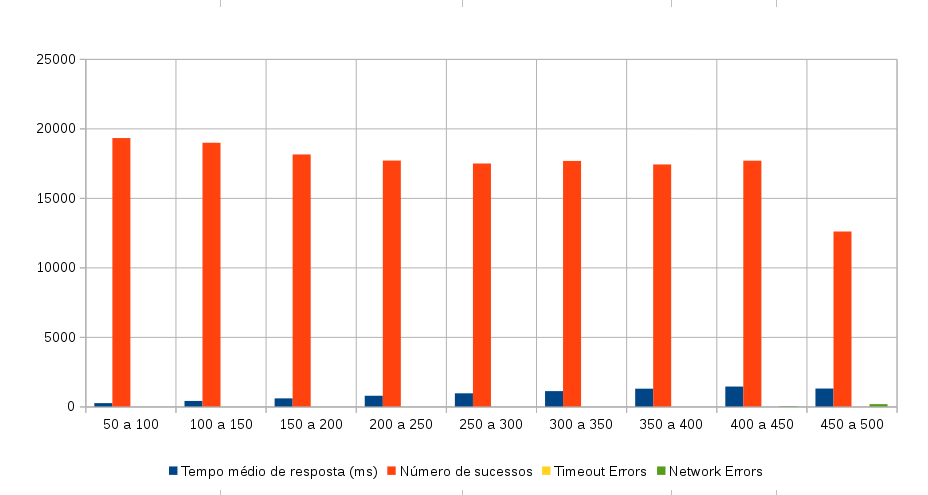
\includegraphics[width=.80\textwidth]{imagem/graficos/grafico_node_plano_de_teste_3.png}
    % Caption centralizada
    \captionsetup[grafico]{justification=centering}
    % Fonte
    \captionfont{\small{\textbf{\\Fonte: Autor}}}
  \end{grafico}

  No gráfico \ref{grafico:teste-mantendo-carga-usuario-node}  observa-se que o tempo de resposta da conexões 
  é muito baixo e o número de sucessos das conexões gira em torno de 17.429 sucessos. Os valores de tempo de resposta e
  número de sucessos somente decrecem quando executa o teste de 450 a 500 usuários. Neste teste houve um alto número de erros 
  de rede o qual influenciou diretamente no número de sucessos.
  
  Neste mesmo gráfico pode-se ver que o o número de erros de tempos de limite é sempre zero. Sendo assim podemos afirmar
  que não houve bloqueio nas operações de consulta a base de dados que poderiam impactar nos próximos testes.
  
  Comparando os dois gráficos \ref{grafico:teste-mantendo-carga-usuario-django} e \ref{grafico:teste-mantendo-carga-usuario-node} é
  visível a eficiência do protótipo em Node.Js pois em todos os campos o resultado obtido superou o primeiro protótipo.
  
  Pode-se concluir que o primeiro protótipo não tem condições de suportar grandes quantidades de usuários conectados ao
  sistema, visto o alto indíce de erros de limite de tempo excedido, baixo número de sucessos e tempo de resposta alto, 
  conforme exposto na tabela \ref{tab:sumario-resultado-plano-teste-a-3}. Para o protótipo Django o número ideal de usuarios
  conectados ao sistema fica em torno de 100 a 150 usuários enquanto em Node.Js tem-se 350 a 400 usuários conectados sem 
  erros.
  
  